%package list
\documentclass{article}
\usepackage[top=3cm, bottom=3cm, outer=3cm, inner=3cm]{geometry}
\usepackage{graphicx}
\usepackage{url}
\usepackage{hyperref}
\usepackage{array}
%\usepackage{multicol}
\newcolumntype{x}[1]{>{\centering\arraybackslash\hspace{0pt}}p{#1}}
\usepackage[numbers,super]{natbib}
\usepackage{pdfpages}
\usepackage{multirow}
\usepackage{cite}
\usepackage{float}
\usepackage[normalem]{ulem}
% %% Own Packages %%
% \usepackage{csquotes}
% \MakeOuterQuote{"}
\usepackage{listings}



%%%%%%%%%%%%%%%%%%%%%%%%%%%%%%%%%%%%%%%%%%%%%%%%%%%%%%%%%%%%%%%%%%%%%%%%%%%%
%%%%%%%%%%%%%%%%%%%%%%%%%%%%%%%%%%%%%%%%%%%%%%%%%%%%%%%%%%%%%%%%%%%%%%%%%%%%
\newcommand{\csemail}{vmachacaa@ulasalle.edu.pe}
\newcommand{\csdocente}{MSc. Vicente Enrique Machaca Arceda}
\newcommand{\cscurso}{Construcción De Software}
\newcommand{\csuniversidad}{Universidad La Salle}
\newcommand{\csescuela}{Escuela Profesional de Ingeniería de Software}
\newcommand{\cspracnr}{07}
\newcommand{\cstema}{Frontend}
%%%%%%%%%%%%%%%%%%%%%%%%%%%%%%%%%%%%%%%%%%%%%%%%%%%%%%%%%%%%%%%%%%%%%%%%%%%%
%%%%%%%%%%%%%%%%%%%%%%%%%%%%%%%%%%%%%%%%%%%%%%%%%%%%%%%%%%%%%%%%%%%%%%%%%%%%


\usepackage[english,spanish]{babel}
\usepackage[utf8]{inputenc}
\AtBeginDocument{\selectlanguage{spanish}}
\renewcommand{\figurename}{Figura}
\renewcommand{\refname}{Referencias}
\renewcommand{\tablename}{Tabla} %esto no funciona cuando se usa babel
\AtBeginDocument{%
	\renewcommand\tablename{Tabla}
}

\usepackage{fancyhdr}
\pagestyle{fancy}
\fancyhf{}
\setlength{\headheight}{30pt}
\renewcommand{\headrulewidth}{1pt}
\renewcommand{\footrulewidth}{1pt}
\fancyhead[L]{\raisebox{-0.2\height}{
\includegraphics[width=4cm]{../../img/lasalle_black.pdf}}}
\fancyhead[C]{}
\fancyhead[R]{\fontsize{7}{7}\selectfont	\csuniversidad \\ \csescuela \\ \textbf{\cscurso} }
\fancyfoot[L]{MSc. Vicente Machaca}
\fancyfoot[C]{\cscurso}
\fancyfoot[R]{Página \thepage}







\begin{document}

\vspace*{10pt}

\begin{center}
    \fontsize{17}{17} \textbf{ Práctica \cspracnr}
\end{center}
%\centerline{\textbf{\underline{\Large Título: Informe de revisión del estado del arte}}}
%\vspace*{0.5cm}


\begin{table}[h]
    \begin{tabular}{|x{4.7cm}|x{4.8cm}|x{4.8cm}|}
        \hline
        \textbf{DOCENTE} & \textbf{CARRERA} & \textbf{CURSO} \\
        \hline
        \csdocente       & \csescuela       & \cscurso       \\
        \hline
    \end{tabular}
\end{table}


\begin{table}[h]
    \begin{tabular}{|x{4.7cm}|x{4.8cm}|x{4.8cm}|}
        \hline
        \textbf{PRÁCTICA} & \textbf{TEMA} & \textbf{DURACIÓN} \\
        \hline
        \cspracnr         & \cstema       & 2 horas           \\
        \hline
    \end{tabular}
\end{table}


\section{Datos de los estudiantes}
\begin{itemize}
    \item Grupo: 1
    \item Integrantes:
          \begin{itemize}
              \item Elvis Andre Cruces Gomez
              \item Yoshiro Milton Miranda Valdivia
              \item José Alfredo Pinto Villamar
          \end{itemize}
\end{itemize}





\section{Implementación para intefaces (GUI)}\label{sec:Intro}
\subsection{Propuesta}
Nuestra propuesta para el frontend se basa, por ahora, en Vuetify nativo, ya que no tuvimos suerte en encontrar un template que se adecuara a nuestras necesidades.

\subsection{Inicio}
\begin{figure}[h]
    \centering
    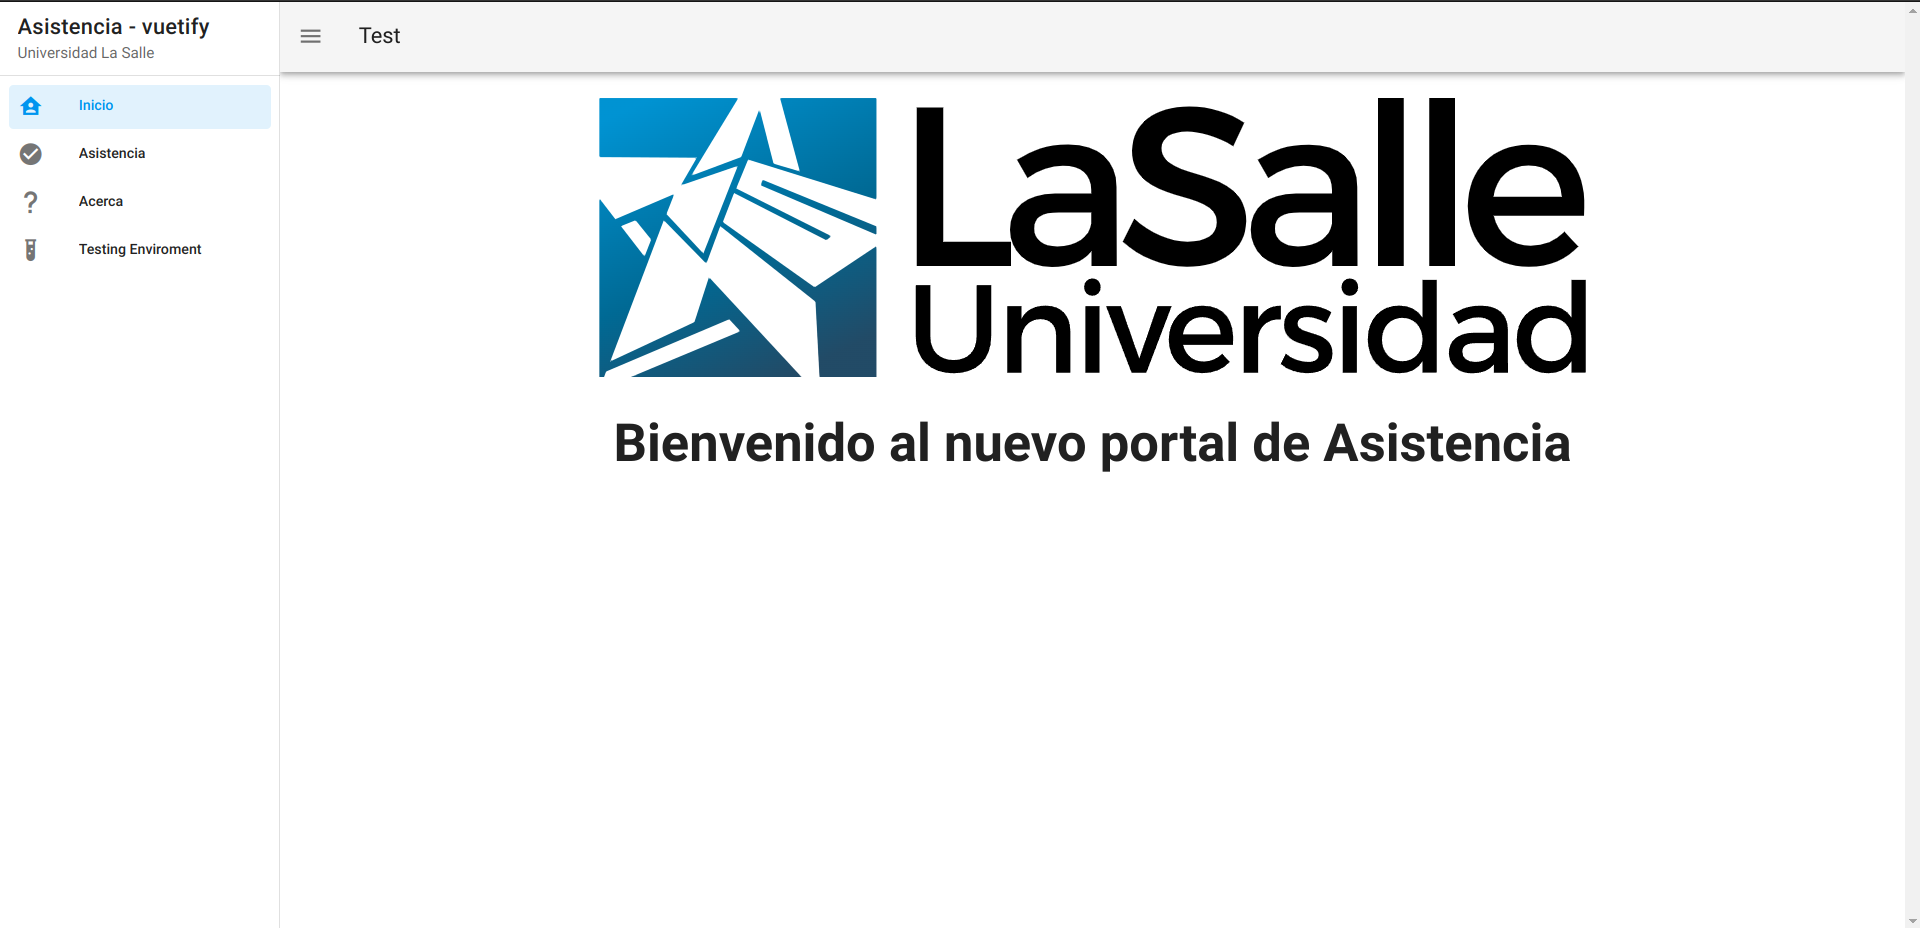
\includegraphics[width=0.8\textwidth]{../img/inicio.png}
    \caption{Pantalla de inicio}
    \label{fig:Inicio}
\end{figure}

Hemos decidido que nuestras vistas puedan ser accedidas por una barra de navegación \textit{navbar} que están en la parte izquierda de la pantalla. En estas podemos acceder encontrar las tablas que tenemos. 

\subsection{User\_type}
\begin{figure}[!h]
    \centering
    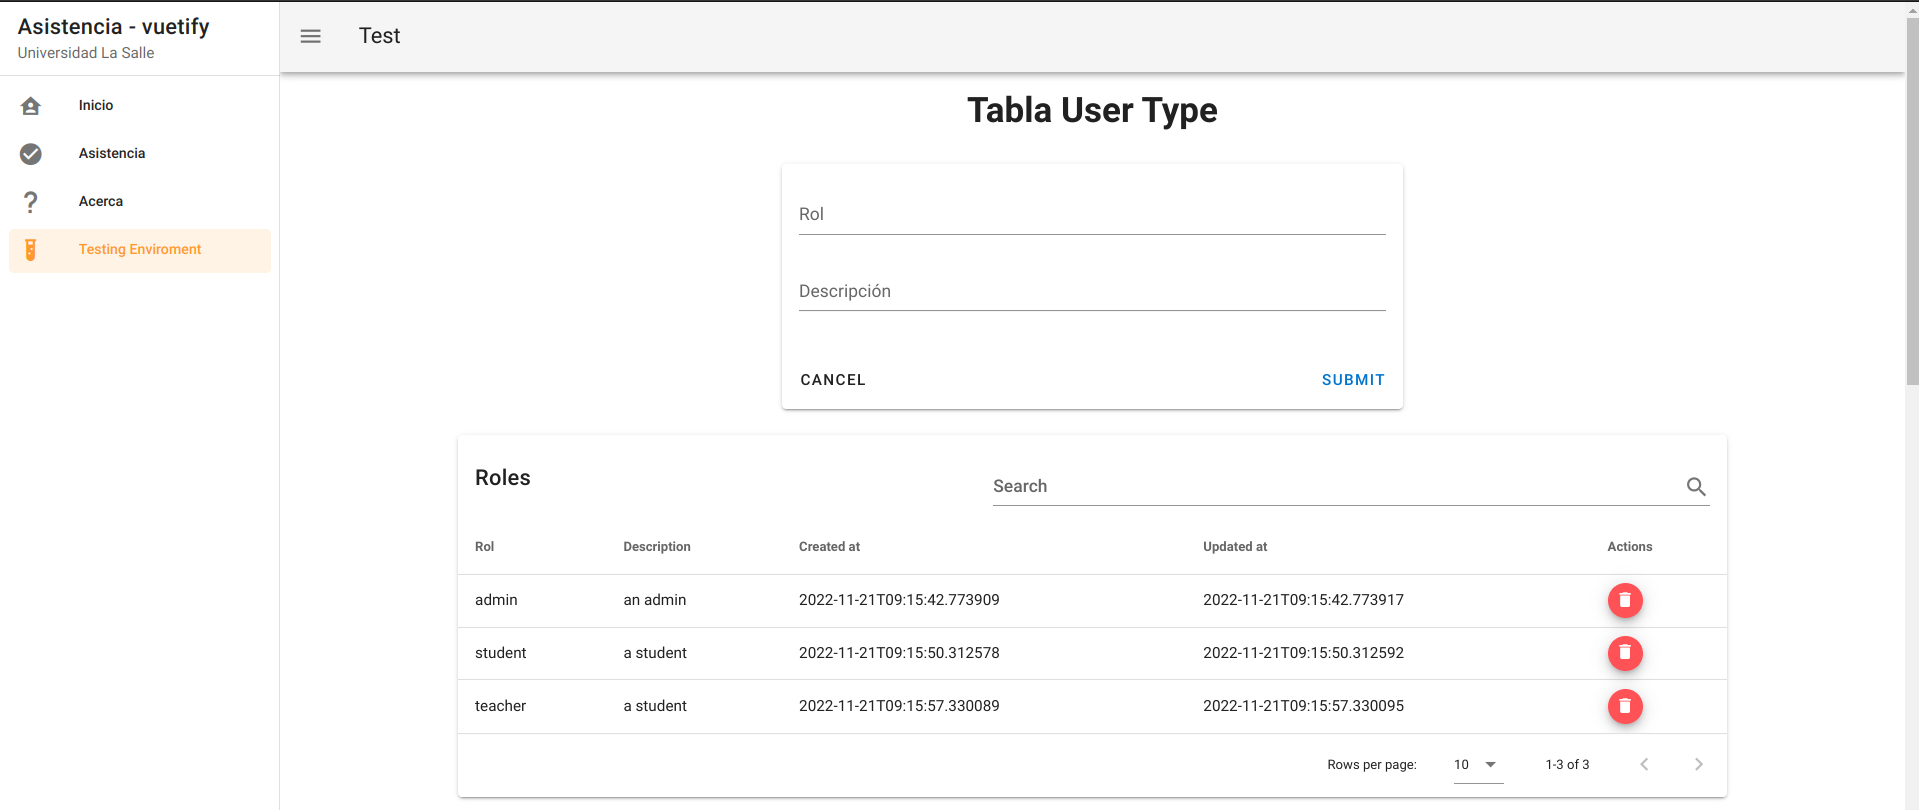
\includegraphics[width=0.8\textwidth]{../img/user_type.png}
    \caption{Pantalla de user\_type}
    \label{fig:user_type}
\end{figure}

En esta pantalla podemos ver la tabla user\_type, en la cual podemos ver los tipos de usuarios que tenemos en nuestra base de datos. En esta pantalla podemos ver los botones de \textit{Agregar}, y \textit{Eliminar}. \pagebreak

\subsection{User}
\begin{figure}[!h]
    \centering
    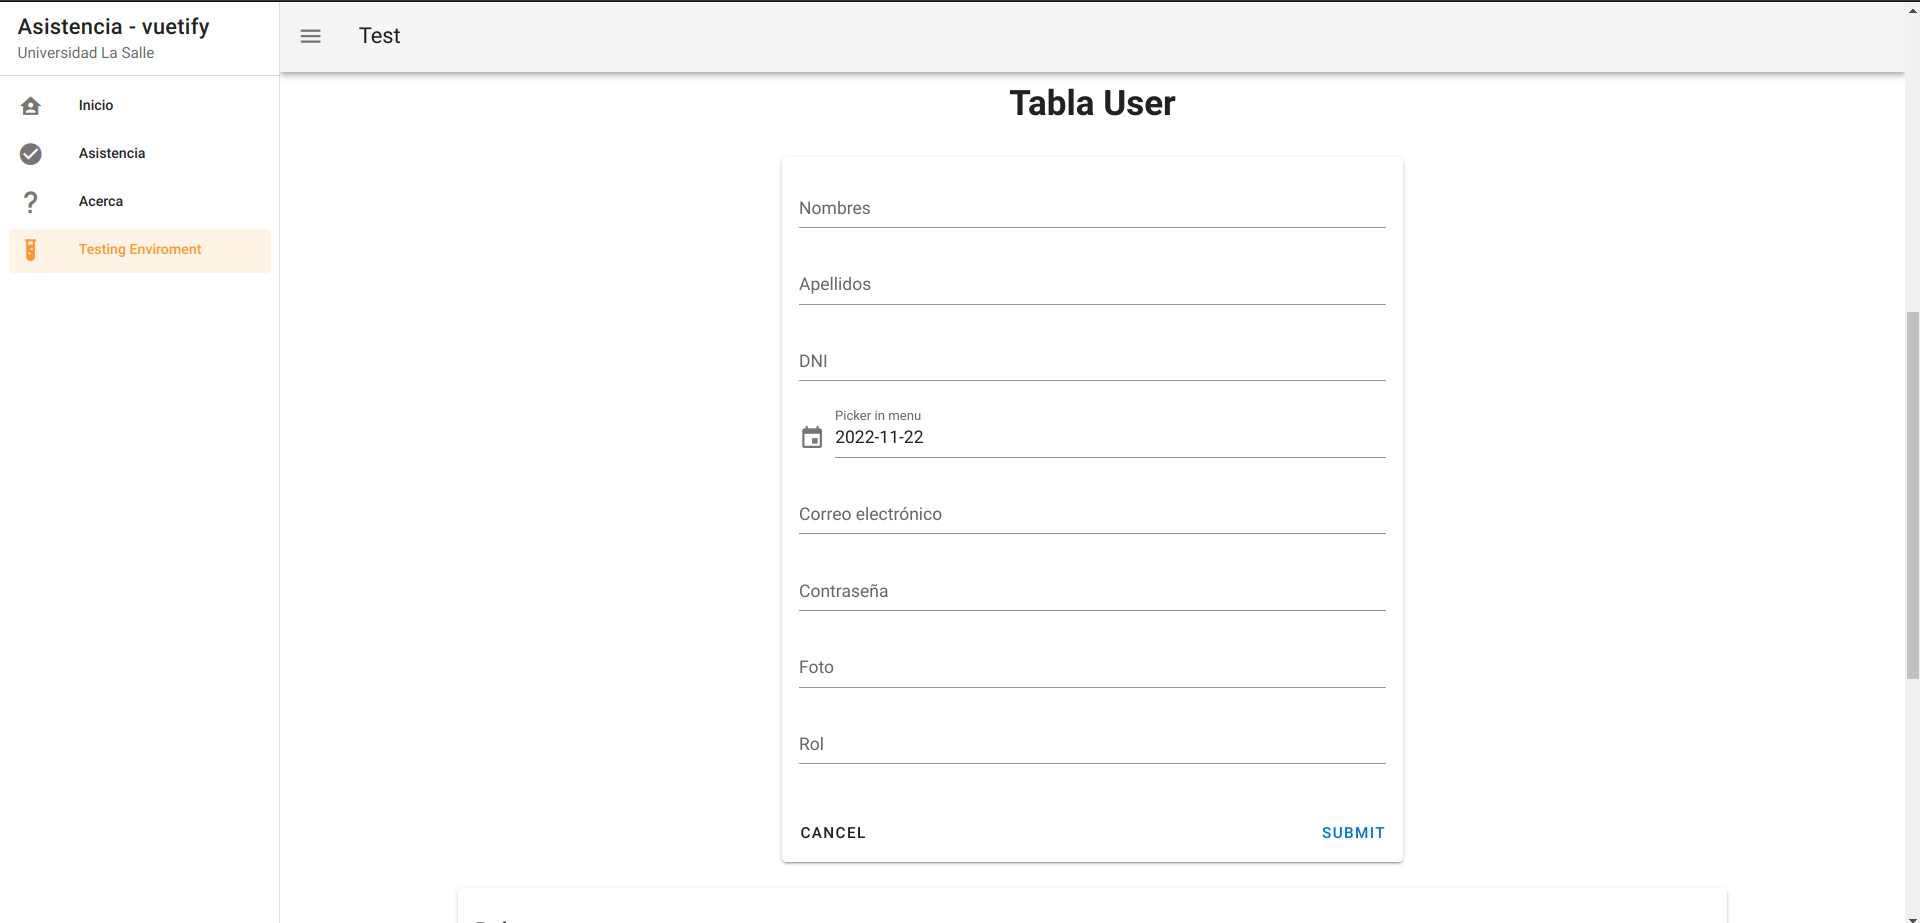
\includegraphics[width=0.8\textwidth]{../img/user.png}
    \caption{Pantalla de user}
    \label{fig:user}
\end{figure}

\begin{figure}[!h]
    \centering
    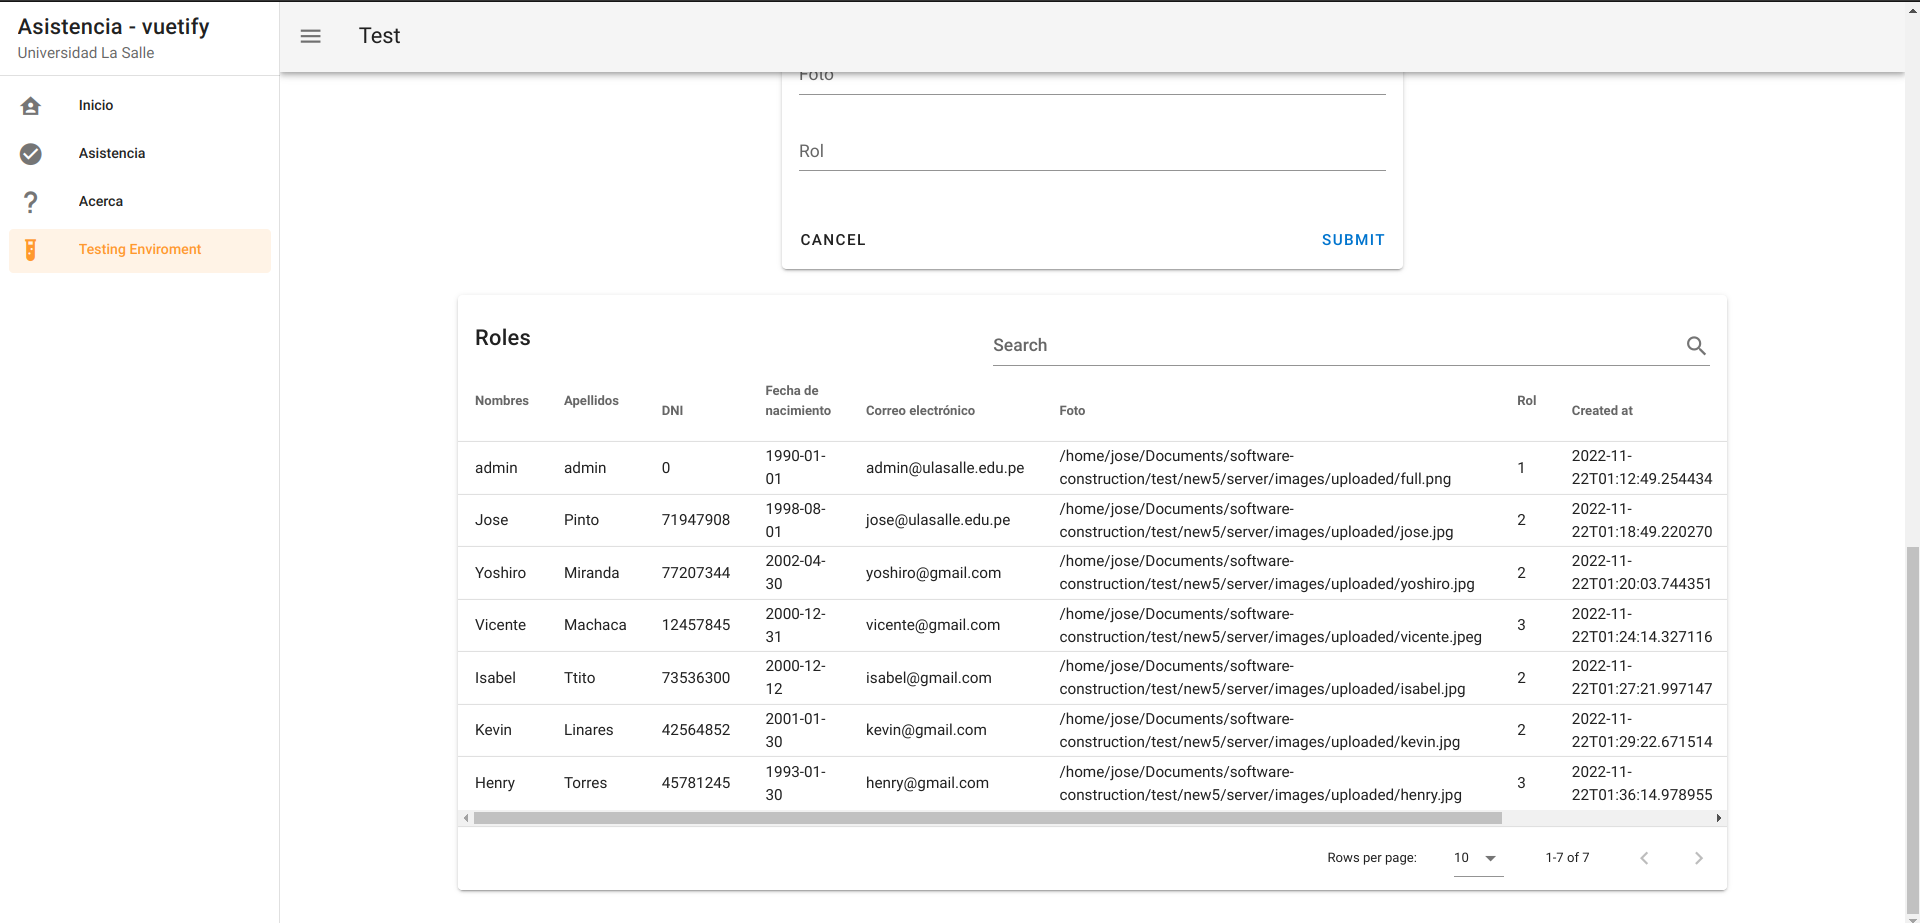
\includegraphics[width=0.8\textwidth]{../img/user2.png}
    \caption{Pantalla de user 2}
    \label{fig:user}
\end{figure}



En esta pantalla podemos ver la tabla user, en la cual podemos ver los usuarios que tenemos en nuestra base de datos. En esta pantalla podemos ver los botones de \textit{Agregar}, y \textit{Eliminar}.
En este caso, hay más campos a los cuales hay que ingresar datos, y no solo \texttt{rawtext} si no tambien, fechas, contraseñas y fotos, por ahora sólo tenemos fechas.






%\clearpage
%\bibliographystyle{apalike}
% \bibliographystyle{IEEEtranN}
% \nocite{*}
% \bibliography{refs.bib}
%\bibliography{bibliography}

\section{Repositorio}\label{sec:Repositorio}
\begin{itemize}
    \item {\color{blue}\href{https://github.com/pintovillamar/software-construction/tree/main/test/new5}{Practica 7}}
\end{itemize}


\end{document}